	% define documentclass
\documentclass[12pt, bibliography=totoc, a4paper, abstractoff, numbers=noenddot]{scrreprt}

% define used packages
\usepackage[left=4.0cm, right=2.0cm, top=3cm, bottom=3cm]{geometry}
\usepackage{bibgerm}
\usepackage[utf8]{inputenc}
\usepackage[T1]{fontenc}
\usepackage{graphicx}
\usepackage[ngerman]{babel}
\usepackage{lmodern}
\usepackage{listings}
\usepackage[numbers]{natbib}
\usepackage{acronym}
\bibliographystyle{alphadin}
\usepackage{float}

\usepackage{lastpage}

% advanced tables
\usepackage{array}

% header and footer
\usepackage{fancyhdr}

% links
\usepackage{url}
%\usepackage{hyperref}

%sourcecode
\usepackage{listings}
\usepackage{color}

% internal links
\usepackage[colorlinks=true ,linkcolor=black,
			anchorcolor=black ,citecolor=black ,filecolor=black,
			menucolor=black ,urlcolor=black]{hyperref}

% mathematical formulas
\usepackage{amsmath, amssymb}

% fancy Diagrams %
\usepackage{tikz}
\usepackage{epstopdf}

% to include images side by side
\usepackage{subfigure}

% for nice bg on title page
\usepackage{eso-pic}
\newcommand\BackgroundPic{%
\put(0,0){%
\parbox[b][\paperheight]{\paperwidth}{%
\vfill
\centering

\includegraphics[width=\paperwidth,height=\paperheight,%
keepaspectratio]{images/Logo_H-BRS_background}%
\vfill
}}}

% define the programming language
\usepackage{listings}
\lstloadlanguages{Java,sh,bash,Haskell,HTML,PHP,XML}
\lstdefinelanguage{console}{
  morekeywords={},
  otherkeywords={warumgehtdasnicht>,\$}
}
\newcommand{\lstsetconsole}
{ \lstset{%language=sh,
        lineskip=-2pt,
        breaklines=true,
        language=console,
        breaklines=true,
        captionpos=b,
        commentstyle=\textit,
        keywordstyle=\bfseries,
        basicstyle=\ttfamily,
        stringstyle=\ttfamily,
        showstringspaces=false,
        frame=single,
        tabsize=2
  }
}
\lstdefinelanguage{scalaconsole}{
  morekeywords={},
  otherkeywords={scala>,\|}
}
\newcommand{\lstsetrepl}
{ \lstset{%language=sh,
        lineskip=-2pt,
        breaklines=true,
        language=scalaconsole,
        breaklines=true,
        commentstyle=\textit,
        keywordstyle=\bfseries,
        basicstyle=\ttfamily,
        stringstyle=\ttfamily,
        showstringspaces=false,
        frame=single,
        tabsize=2
  }
}
\newcommand{\lstsetjava}{
 \lstset{language=Java,
        breaklines=true,
        commentstyle=\textit,
        keywordstyle=\bfseries,
        basicstyle=\ttfamily,
        stringstyle=\ttfamily,
        showstringspaces=false,
        frame=single,
        captionpos=b,
        tabsize=2,
        literate=
        %linewidth=\textwidth,captionpos=b
        %numbers=left, stepnumber=5, numbersep=10pt
 }
}
\lstdefinelanguage{scala}{
  morekeywords={abstract,case,catch,class,def,%
    do,else,extends,false,final,finally,%
    for,forSome,if,implicit,import,lazy,match,mixin,%
    new,null,object,override,package,%
    private,protected,requires,return,sealed,%
    super,this,throw,trait,true,try,%
    type,val,var,while,with,yield},
  otherkeywords={_,:,=,=>,<-,<\%,<:,>:,\#,@},
  sensitive=true,
  morecomment=[l]{//},
  morecomment=[n]{/*}{*/},
  morestring=[b]",
  morestring=[b]',
  morestring=[b]"""
}
\newcommand{\lstsetscala}{
 \lstset{language=scala,
        breaklines=true,
        commentstyle=\textit,
        keywordstyle=\bfseries,
        basicstyle=\ttfamily,
        stringstyle=\ttfamily,
        showstringspaces=false,
        frame=single,
        tabsize=2
        %%linewidth=\textwidth,captionpos=b
        %numbers=left, stepnumber=5, numbersep=10pt
 }
}
\newcommand{\lstsethtml}{
 \lstset{language=HTML,
        breaklines=true,
        commentstyle=\textit,
        keywordstyle=\bfseries,
        basicstyle=\ttfamily,
        stringstyle=\ttfamily,
        showstringspaces=false,
        frame=single,
        tabsize=2
        %%linewidth=\textwidth,captionpos=b
        %numbers=left, stepnumber=5, numbersep=10pt
 }
}
\newcommand{\lstsetphp}{
 \lstset{language=PHP,
        breaklines=true,
        commentstyle=\textit,
        keywordstyle=\bfseries,
        basicstyle=\ttfamily,
        stringstyle=\ttfamily,
        showstringspaces=false,
        frame=single,
        tabsize=2
        %%linewidth=\textwidth,captionpos=b
        %numbers=left, stepnumber=5, numbersep=10pt
 }
}
\lstnewenvironment{code}
    {\lstset{}%
      \csname lst@SetFirstLabel\endcsname}
    {\csname lst@SaveFirstLabel\endcsname}
\newcommand{\lstsethaskell}{
    \lstset{
      language=Haskell,
      commentstyle=\textit,
      keywordstyle=\bfseries,
      basicstyle=\ttfamily,
      stringstyle=\ttfamily,
      showstringspaces=false,
      frame=single,
      flexiblecolumns=false,
      basewidth={0.5em,0.45em},
      literate={+}{{$+$}}1 {/}{{$/$}}1 {*}{{$*$}}1 {=}{{$=$}}1
               {==}{{$==$}}2 %{!=}{{$\not\equiv$}}2
               {>}{{$>$}}1 {<}{{$<$}}1 {\\}{{$\lambda$}}1
               {\\\\}{{\char`\\\char`\\}}1
               {->}{{$\rightarrow$} }2 {>=}{{$\geq$}}2 {<-}{{$\leftarrow$}}2
               {<=}{{$\leq$}}2 {=>}{{$\Rightarrow$} }2
               {\ .}{{$\circ$}}2 {\ .\ }{{$\circ$}}2 {(.)}{({$\circ$})}2
               {>>}{{>>}}2 {>>=}{{>>=}}2
               {|}{{$\mid$}}1
    }
}
\lstdefinelanguage{JavaScript}{
  keywords={typeof, new, true, false, catch,%
    function, return, null, catch, switch, var,%
    if, in, while, do, else, case, break},
  ndkeywords={class, export, boolean, throw, implements, import, this},
  sensitive=false,
  comment=[l]{//},
  morecomment=[s]{/*}{*/},
  morestring=[b]',
  morestring=[b]"
}
\newcommand{\lstsetjavascript}{
  \lstset{
		language=JavaScript,
		breaklines=true,
		commentstyle=\textit,
		basicstyle=\ttfamily,
		keywordstyle=\bfseries,
		stringstyle=\ttfamily,
		showstringspaces=false,
		frame=single,
		tabsize=2
  }
}
\newcommand{\lstsetxml}{
 \lstset{language=XML,
        breaklines=true,
        commentstyle=\sffamily,
        keywordstyle=\bfseries,
        basicstyle=\sffamily,
        showstringspaces=false,
        stringstyle=\ttfamily,
        frame=single,
        tabsize=2,
        literate=
        %linewidth=\textwidth,captionpos=b
        %numbers=left, stepnumber=5, numbersep=10pt
 }
}
\lstdefinelanguage{CSharp}{
 morekeywords = {abstract,event,new,struct,as,explicit,%
    null,switch,base,extern,object,this,bool,false,%
    operator,throw,break,finally,out,true,byte,fixed,%
    override,try,case,float,params,typeof,catch,for,%
    private,uint,char,foreach,protected,ulong,checked,%
    goto,public,unchecked,class,if,readonly,unsafe,%
    const,implicit,ref,ushort,continue,in,return,using,%
    decimal,int,sbyte,virtual,default,interface,sealed,%
    volatile,delegate,internal,short,void,do,is,sizeof,%
    while,double,lock,stackalloc,else,long,static,%
    enum,namespace,string,partial},
  morecomment = [l]{//},
  morecomment = [l]{///},
  morecomment = [s]{/*}{*/},
  morestring=[b]",
  sensitive = true
}
\newcommand{\lstsetcsharp}{
 \lstset{language=csharp,
        breaklines=true,
        commentstyle=\sffamily,
        basicstyle=\sffamily,
        keywordstyle=\bfseries,
        stringstyle=\ttfamily,
        showstringspaces=false,
        frame=single,
        tabsize=2
        %%linewidth=\textwidth,captionpos=b
        %numbers=left, stepnumber=5, numbersep=10pt
 }
}
\lstdefinelanguage{FSharp}{
  morekeywords={abstract,and,as,assert,base,begin,%
    class,default,delegate,do,done,downcast,downto,%
    elif,else,end,exception,extern,false,finally,for,fun,%
    function,if,in,inherit,inline,interface,internal,lazy,%
    let,match,member,module,mutable,namespace,%
    new,not,null,of,open,or,override,private,public,rec,%
    return,static,struct,then,to,true,try,type,upcast,use,%
    val,void,when,while,with,yield,asr,land,lor,lsl,lsr,lxor,%
    mod,sig,atomic,break,checked,component,const,%
    constraint,constructor,continue,eager,event,external,%
    fixed,functor,global,include,method,mixin,object,%
    parallel,process,protected,pure,sealed,tailcall,trait,virtual,volatile},     
  sensitive=false,
  morecomment=[l][\color{greencomments}]{///},
  morecomment=[l][\color{greencomments}]{//},
  morecomment=[s][\color{greencomments}]{{(*}{*)}},
  morestring=[b]"
}
\newcommand{\lstsetfsharp}{
 \lstset{language=fsharp,
        breaklines=true,
        commentstyle=\sffamily,
        basicstyle=\sffamily,
        keywordstyle=\bfseries,
        stringstyle=\ttfamily,
        showstringspaces=false,
        frame=single,
        tabsize=2
        %%linewidth=\textwidth,captionpos=b
        %numbers=left, stepnumber=5, numbersep=10pt
 }
}

%set default pagestyle
\pagestyle{empty}

\setlength{\parindent}{0pt}
\setlength{\parskip}{12pt}

% #####
% #
% # START config area
% #
% #####

\newcommand{\HEADER}[0]{H-BRS, WS 2016 / 2017}
\newcommand{\PAGENUMBERS}[0]{\pagemark}
\newcommand{\DATE}[0]{05.12.2016}

\newcommand{\AUTHOR}[0]{Franz-Dominik Dahmann, Jan Eric M\"uller, Thomas Zok}
\newcommand{\MATNR}[0]{entf\"allt}
\newcommand{\STREET}[0]{ }
\newcommand{\ZIP}[0]{ }
\newcommand{\TOWN}[0]{ }

\newcommand{\REFERENT}[0]{Prof. Dr. Knolle} 
\newcommand{\KOREFERENT}[0]{B. Mager}

\newcommand{\TITLE}[0]{MongoDB als Datenbank für Document Stores}
\newcommand{\COURSE}[0]{Studiengang MCS}
\newcommand{\TYPE}[0]{Schemalose Datenbank}
\newcommand{\COMPLETION}[0]{Master of Science}

% #####
% #
% # END config area
% #
% #####

% Hurenkinder und Schusterjungenregelung
\clubpenalty=100000
\widowpenalty=100000
\displaywidowpenalty=100000

% starting the document
\begin{document}

% set pagenumbering to roman(I II III IV)
\pagenumbering{Roman}
% input the title
% #####
% #
% # This is the titlelayout from Prof. Dr. Harm Knolle 
% # (Hochschule Bonn-Rhein-Sieg)
% #  
% #####

% #####
% #
% # Default layout
% #
% #####

\AddToShipoutPicture*{\BackgroundPic}

\begin{titlepage}
  \begin{center}
  	
\includegraphics[scale=1]{./images/Logo_H-BRS.jpg}
  \end{center}
  \vspace{40pt}
  \sffamily
  \begin{tabular}{|l>{\raggedright\hspace{0pt}\arraybackslash}p{15cm}}
    & \\
    & \large\textbf{\TYPE}\\[\baselineskip]
    & \huge\textbf{\TITLE}\\[\baselineskip]
    & \textbf{Falls erforderlich: Zur Erlangung des akademischen Grades eines}\\ 
    & \COMPLETION\\
    & - \COURSE\ -\\
    & \\
  \end{tabular}
  \vfill
  \begin{tabular}{ll@{}}
    & Fachbereich Informatik\\[\baselineskip]
    &   Referent: \REFERENT\\[\baselineskip]
    &   Falls erforderlich: Korreferent: \KOREFERENT\\[\baselineskip]
    & \\[\baselineskip]
    & eingereicht von:\\[\baselineskip]
    & \AUTHOR\\[\baselineskip]
    & Matr.-Nr. \MATNR\\[\baselineskip]
    & \STREET\\[\baselineskip]
    & \ZIP \ \TOWN\\[\baselineskip]
    & \\[\baselineskip]
    & Sankt Augustin, den \DATE\\[\baselineskip]
  \end{tabular}
\end{titlepage}


% load the preamble
%% \renewcommand\abstractname{Danksagung}
\begin{abstract}
\section*{Vorwort}\markboth{Vorwort}{}
  \addcontentsline{toc}{chapter}{Vorwort}Lorem ipsum dolor sit amet, consetetur sadipscing elitr, sed diam nonumy eirmod tempor invidunt ut labore et dolore magna aliquyam erat, sed diam voluptua. At vero eos et accusam et justo duo dolores et ea rebum. Stet clita kasd gubergren, no sea takimata sanctus est Lorem ipsum dolor sit amet. Lorem ipsum dolor sit amet, consetetur sadipscing elitr, sed diam nonumy eirmod tempor invidunt ut labore et dolore magna aliquyam erat, sed diam voluptua. At vero eos et accusam et justo duo dolores et ea rebum. Stet clita kasd gubergren, no sea takimata sanctus est Lorem ipsum dolor sit amet. Lorem ipsum dolor sit amet, consetetur sadipscing elitr, sed diam nonumy eirmod tempor invidunt ut labore et dolore magna aliquyam erat, sed diam voluptua. At vero eos et accusam et justo duo dolores et ea rebum. Stet clita kasd gubergren, no sea takimata sanctus est Lorem ipsum dolor sit amet. 

Duis autem vel eum iriure dolor in hendrerit in vulputate velit esse molestie consequat, vel illum dolore eu feugiat nulla facilisis at vero eros et accumsan et iusto odio dignissim qui blandit praesent luptatum zzril delenit augue duis dolore te feugait nulla facilisi. Lorem ipsum dolor sit amet, consectetuer adipiscing elit, sed diam nonummy nibh euismod tincidunt ut laoreet dolore magna aliquam erat volutpat. 

Ut wisi enim ad minim veniam, quis nostrud exerci tation ullamcorper suscipit lobortis nisl ut aliquip ex ea commodo consequat. Duis autem vel eum iriure dolor in hendrerit in vulputate velit esse molestie consequat, vel illum dolore eu feugiat nulla facilisis at vero eros et accumsan et iusto odio dignissim qui blandit praesent luptatum zzril delenit augue duis dolore te feugait nulla facilisi. 

Nam liber tempor cum soluta nobis eleifend option congue nihil imperdiet doming id quod mazim placerat facer possim assum. Lorem ipsum dolor sit amet, consectetuer adipiscing elit, sed diam nonummy nibh euismod tincidunt ut laoreet dolore magna aliquam erat volutpat. Ut wisi enim ad minim veniam, quis nostrud exerci tation ullamcorper suscipit lobortis nisl ut aliquip ex ea commodo consequat. 

Duis autem vel eum iriure dolor in hendrerit in vulputate velit esse molestie consequat, vel illum dolore eu feugiat nulla facilisis. 
\end{abstract}


% loads the fancy pagestyle for register part
% set the pagestyle to fancy
\pagestyle{fancy}

\fancyhf{}% clear all fields
  % define the header
  \fancyhead[L]{\leftmark}% left header
  \fancyhead[R]{\HEADER}% right header
  \renewcommand{\headrulewidth}{0.4pt}% top line

  % define the footer
  \fancyfoot[L]{\AUTHOR}% left footer
  \fancyfoot[R]{\pagemark}% right footer
  \renewcommand{\footrulewidth}{0.6pt}% bottom line

  % redefine the chaptermark to have '1. Chaptername' and not 'CHAPTER 1.
  % CHAPTERNAME'
  \renewcommand{\chaptermark}[1]{\markboth{\thechapter.\ #1}{}}

% override the plain style
\fancypagestyle{plain}{%
\fancyhf{}% clear all fields
  % define the header
  \renewcommand{\headrulewidth}{0.0pt}% top line

  % define the footer
  \fancyfoot[L]{\AUTHOR}% left footer
  \fancyfoot[R]{\pagemark}% right footer
  \renewcommand{\footrulewidth}{0.6pt}% bottom line
}


% create the registers
\tableofcontents\newpage

% set pagenumbering to arabic(1 2 3 4)
\pagenumbering{arabic}
% loads the fancy pagestyle for main part
% set the pagestyle to fancy
\pagestyle{fancy}

\fancyhf{}% clear all fields
  % define the header
  \fancyhead[L]{\leftmark}% left header
  \fancyhead[R]{\HEADER}% right header
  \renewcommand{\headrulewidth}{0.4pt}% top line

  % define the footer
  \fancyfoot[L]{\AUTHOR}% left footer
  \fancyfoot[R]{\PAGENUMBERS}% right footer
  \renewcommand{\footrulewidth}{0.6pt}% bottom line

  % redefine the chaptermark to have '1. Chaptername' and not 'CHAPTER 1.
  % CHAPTERNAME'
  \renewcommand{\chaptermark}[1]{\markboth{\thechapter.\ #1}{}}

% override the plain style
\fancypagestyle{plain}{%
\fancyhf{}% clear all fields
  % define the header
  \renewcommand{\headrulewidth}{0pt}% top line

  % define the footer
  \fancyfoot[L]{\AUTHOR}% left footer
  \fancyfoot[R]{\PAGENUMBERS}% right footer
  \renewcommand{\footrulewidth}{0.6pt}% bottom line
}

%----------------------------------OUR SHIT--------------------------
%Vorwort
\chapter{Vorwort}
\cite{edlich01}
\cite{sadalage01}
\cite{redmont01}
\cite{Jing01}
\cite{Bogdan01}
\cite{Meier01}
\cite{Fasel01}
\cite{Meier02}
\cite{Fasel02}
\cite{Boicea01}
\cite{Parker01}
\cite{Abramova01}
\cite{Faraj01}
\cite{Shakuntala01}
\cite{Hows01}
\cite{fowler01}
\cite{harrison01}
Zuordnungen von Aufgabenpaketen auf die Gruppenmitglieder. Diese Zuordnung fließt insbesondere dann in die Einzelbewertung mit ein, wenn eine homogene Gruppenleistung nur schwer festgestellt werden kann.
In der eidesstattlichen Erklärung (s.u.) gibt es einen Verweis auf das Vorwort.
Die Zuordnung kann tabellarisch erfolgen. Damit die Tabelle nicht zu breit wird, definieren Sie einfach einen DreiLetterCode pro Gruppenmitglied
Für die folgenden (falls Vorhanden) Abschnitte (Zeilen) ...

    Ausgewählte technologische Grundlagen
    Ausgewählte Persistenzmodelle
    Ausgewählte Persistenzsysteme und Big Data Frameworks
        Vorstellung des Systems
        Installation des Systems
        Ad-Hoc-Anwendung des Systems (CRUD)
        Implementierung der Beispiel-Datenbank
    Ausgewählte Anwendungsszenarien
        Spezifikation des Anwendungsszenarios
        Spezifikation der konkreten Anwendung
        Implementierung der Anwendung

... werden jeweils die folgenden Zuordnungen (Spalten) erwartet:

    Hauptverantwortlicher schriftliche Ausarbeitung
    Hauptverantwortlicher praktische Umsetzung am Rechner
    Hauptverantwortlicher Erstellung Vortrag
    Hauptverantwortlicher Vortrag vorgetragen
\chapter{Ausgewählte Persistenzmodelle}
\section{Key-Value Stores}
\subsection{Einleitung}
Key-Value Stores oder Key-Value Datenbanken sind eine der einfachsten Formen der NoSQL Datenbanken. Sie können beliebige Werte (Englisch: Values) unter einem definierbaren Key persistieren und über diesen selektieren. Dabei können sie mit einem herkömmlichen relationalen Datenbanksystem (RDBS) verglichen werden in welchem die Tabellen nur zwei Attribute besitzen: eine ID- und eine Value-Spalte \cite{sadalage01}. Im Unterschied zu dieser relationalen Datenbank erwarten Key-Value Stores keinen Datentyp für den Value. Hier können beliebige Werte als blob gespeichert werden. Auch können Key-Value Datenbanken weder Relationen oder Beziehungen zwischen den Einträgen herstellen. Für die Semantik, Korrektheit der Werte, Beziehungen o.ä., ihre Verwendung, welcher Datentyp vorliegt und etwaiges Fehlerhandling ist allein die Anwendung, welche die Datenbank nutzt, verantwortlich. Dieses sehr grundlegende Verhalten soll eine möglichst hohe Performance und Skalierbarkeit ermöglichen. 

\subsection{Eigenschaften}
Einige Key-Value Stores gehen einen Schritt weiter und können das zu speichernde Aggregat differenzieren. So kann Redis beispielsweise Listen, Sets oder Hashes speichern und unterstützt einfache Operationen auf diesen Datenstrukturen. Somit verschwimmt in der Praxis der Unterschied zwischen Key-Value und Document Stores bei einigen Vertretern sehr.

Im Folgenden werden einige Eigenschaften von Key-Value Stores näher betrachtet und aufgezeigt wie diese sich von einem Standard RDBS unterscheiden.

\subsubsection{Konsistenz}
Da die Key-Value Datenbank Änderungen des Values nicht bestimmen kann, kann die Konsistenz somit nur über den Key und die damit verbundenen Operationen get, put oder delete gewährt werden \cite{sadalage01}. 

In verteilten System wird häufig die \textit{eventually consistent} Eigenschaft angewendet. 

\subsubsection{Transaktionen}
Für Transaktionen gibt es in der NoSQL Welt keine einheitliche Spezifikation. Jeder Anbieter von Key-Value Stores implementiert diese anders, Riak benutzt hier beispielsweise das Quorum-Konzept \cite{sadalage01}.

\subsubsection{Query-Eigenschaften}
Da sich Key-Value Datenbanken nicht für den gespeicherten Value interessieren kann man Queries nur auf den Key ausführen. Auf Grund dieses sehr einfachen Handlings sind Key-Value Stores nicht für Anwendungen geeignet, welche über den Inhalt filtern oder suchen müssen. Hier muss die Anwendung wissen welche Daten unter welchem Key zu finden sind und welchen Key sie aufrufen möchte. Da nicht immer der Fall eintritt, dass der Key zu einem Datum bekannt ist, stellen manche Key-Value Datenbanken allerdings eine Suchfunktionalität oder die Möglichkeit der Indexierung bereit, damit nicht jeder Datensatz von der Anwendung geladen und einzeln durchsucht werden muss \cite{sadalage01}. 

\subsubsection{Struktur der Daten}
Wie bereits erwähnt können in Key-Value Datenbanken verschiedenste Datentypen wie blob, text, JSON, XML oder weitere gespeichert werden, da die Datenbank sich um diese Werte nicht weiter kümmert. Bestimmte Datenbanken, wie beispielsweise Riak können einem Request einen Content-Type übergeben womit diese weiß wie sie die Daten behandeln soll \cite{sadalage01}.

\subsubsection{Skalierbarkeit}
Um die Performance zu erhöhen arbeiten die meisten Key-Value Stores mit „Sharding“. Hierbei entscheidet der Wert des Keys auf welchem Knoten bzw. Shard der Datenbank ein Datum gespeichert wird. So werden beispielsweise alle Keys, welche mit g beginnen auf einem anderen Shard gespeichert als solche, die mit a oder einem nummerischen Wert beginnen. Zusätzliche Shards können sehr einfach ergänzt werden. Um hierbei die Konsistenz nicht zu gefährden, sollte ein Knoten ausfallen, können diese Shards repliziert werden. Die einzelnen Key-Value Datenbanken bieten hierbei verschiedene Möglichkeiten an. So kann bei Riak angegeben werden, wie viele Knoten bei Schreib- und Lesezugriffen mindestens beteiligt sein müssen damit die Transaktion als erfolgreich gilt. 

\subsection{Abgrenzung zu Document-Stores}
Sehr ähnlich, Unterschied: Das Aggregat muss eine bestimmte Struktur haben/ von bestimmtem Typ sein
Mit Document Stores sind Abfragen auf Attribute möglich. Hier nur per Key.
In der Praxis verschwimmt die klare Trennung.
Unfertig …

\subsection{Anwendungsfälle}
Da die Keys in den Key-Value Stores von der Anwendung verwaltet werden, können diese verschiedenen Charakter haben. Eine Möglichkeit ist diese Keys durch einen bestimmten Algorithmus, zum Beispiel eine Hashfunktion, zu generieren. Man kann den Key auch durch Benutzerinformationen, wie Email-Adresse oder User-ID generieren. Alternativ kann dieser auch aus einem Zeitstempel oder anderen Attributen erstellt werden. Dies macht Key-Value Stores attraktiv um Session Informationen, Einkaufswagen im Online-Shopping, Benutzerprofile oder Protokolldateien abzuspeichern, da diese Daten unter einem eindeutigen Key als ein Objekt gespeichert werden \cite{sadalage01}. 

Anwendungsfälle in welchen Key-Value Stores weniger gut geeignet sind:
\begin{itemize}
\item bei Abhängigkeiten oder Beziehungen zwischen den Daten wie sie in herkömmlichen RDBS zu finden sind.
\item bei \textit{Multioperation Transactions}, in welchen bei einem Fehler die restlichen Operationen zurückgedreht werden müssten.
\item bei (Such-)Anfragen, welche den Inhalt der Daten betreffen.
\item bei Operationen, die sich auf mehrere Datensätze zum gleichen Zeitpunkt beziehen, da eine Operation in einem Key-Value Store auf einen Key beschränkt ist.
\end{itemize}

\subsection{Bewertung}
Key-Value Stores ziehen ihren großen Vorteil aus der Einfachheit ihrer Implementierung. Diese ermöglicht ihnen eine hohe Performance. Hierbei verzichten sie absichtlich auf Funktionen, wie Beziehungen, feste Datentypen und die Möglichkeit Abfragen auf jedes Attribut eines Datensatzes zu stellen, die durch die relationale Datenbankwelt bekannt geworden sind. 

\section{Document Stores}
\subsection{Einleitung}
Document-Stores speichern strukturierte Daten in Datensätzen, die Dokumente genannt werden. Grundsätzlich vereinigen sie die Schemafreiheit von Key-Value-Stores mit der Möglichkeit zur Strukturierung der gespeicherten Daten. Somit lassen sich Document-Stores als Erweiterung von Key-Value Stores betrachten. Vorteil hierbei ist, dass es bei Document-Stores im Gegensatz zu Key-Value Stores möglich ist, komplexere auf den Inhalt (die Attribute) der Dokumente gerichtete Abfragen zu stellen. Dies ist bei Key-Value-Stores nicht möglich.

\subsection{Eigenschaften}
Bei der Betrachtung von Document-Stores bezieht sich das Wort \grqq document\grqq auf die hierarchische Struktur der abgespeicherten Daten. Die hier betrachteten Dokumente bestehen jedoch lediglich aus binären Daten oder einfachem Text. Ferner kann es sich um Semi-strukturierte Daten wie JSON oder XML handeln. Während ältere Document-Stores auf XML setzten, ist bei neueren Document-Stores das JSON ähnliche BSON üblich. 
\\

In einer Document-Store basierten NoSQL-Datenbank ist es möglich beliebigen Daten zu speichern, ohne das die Datenbank im Vorfeld Wissen über die Struktur der Daten hat oder weiß was die Daten bedeuten. Gegenüber relationalen Datenbanken bietet dies den Vorteil, dass das Datenbankschema bei kleinen Änderungen nicht durch gr\"o\ss{}ere \"Anderungen ver\"andert werden muss \cite{harrison01}. \\

In einer Document-Store Datenbank ist folgende Hierarchie typischerweise anzutreffen:
\begin{itemize}
\item Ein Dokument ist eine Grundeinheit für das speichern von Daten. Sie ist zu vergleichen mit einer Zeile einer Relationalen Datenbank.
\item Ein Dokument besteht aus einem oder mehreren Key-Value Paaren, und kann weitere Dokumente und Arrays enthalten. die Arrays können wiederum ebenfalls Dokumente enthalten, was eine komplexere Strukturierung ermöglicht.
\item eine Sammlung oder ein Data Bucket ist ein Set von Dokumenten, die einen Zweck teilen. Dies ist äquivalent zu einer relationalen Tabelle. Hier ist jedoch relevant zu erwähnen, dass die Dokumente hier nicht vom gleichen Typ sein müssen, auch wenn es üblich ist, dass solche Dokumente die gleiche Art von Information darstellen \cite{harrison01}.
\end{itemize}

\subsection{Datenmodell}
Im Zentrum des Datenmodells der Document-Stores stehen die Documents, die eine hierarchische Struktur aufweisen. So kann ein Dokument auf viele weitere Dokumente verweisen. Dies ist möglich, da ein Dokument Listen enthalten kann. 
\\

Wie bereits erwähnt ist es möglich mithilfe von Document-Stores ein relationales Schema nachzubilden. Dies ist jedoch häufig nicht sinnvoll, da es größere Vorteile bringt die Dokumente in kleineren Sammlungen zusammenzufassen und in eingebetteten Dokumente die größte Detailstufe zu bieten \cite{harrison01}. 
\\

Sei \ref{fig:doc2} die Darstellung einer relationalen Datenbank mit Filmen und Schauspielern.
\begin{figure}[H]
	\centering
	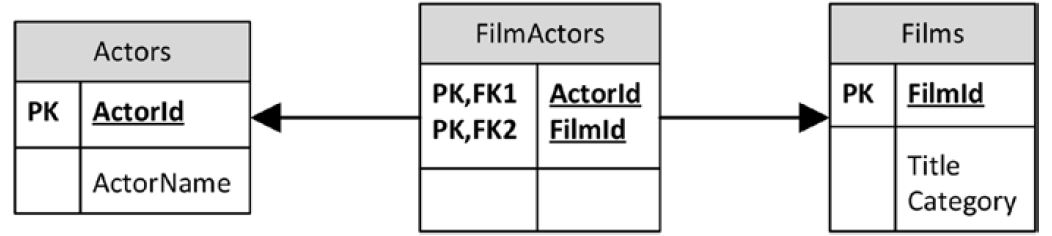
\includegraphics[scale=0.4]{images/01docstores_2.jpg} 
	\caption{Beispiel eines JSON-Dokuments}\label{fig:doc2}
\end{figure}
In einer relationalen Datenbank würde es eine Tabelle mit Filmen und eine Tabelle mit Schauspielern geben, die zu einer gemeinsamen Tabelle gejoint werden würden um anzuzueigen welcher Schauspieler bei welchem Film mitgewirkt hat. Mithilfe von Document-Stores wäre dieses Schema so auch möglich, jedoch gibt es hierfür einen besseren Ansatz. Da Document-Stores grundsätzlich keine Join-Operationen ermöglichen und Entwickler es bevorzugen wenn die JSON Strukturen sich nah an dem objektorientierten Programmentwurf orientieren, bietet sich ein Entwurf nach \ref{fig:doc1} eher an \cite{harrison01}.
\begin{figure}[H]
	\centering
	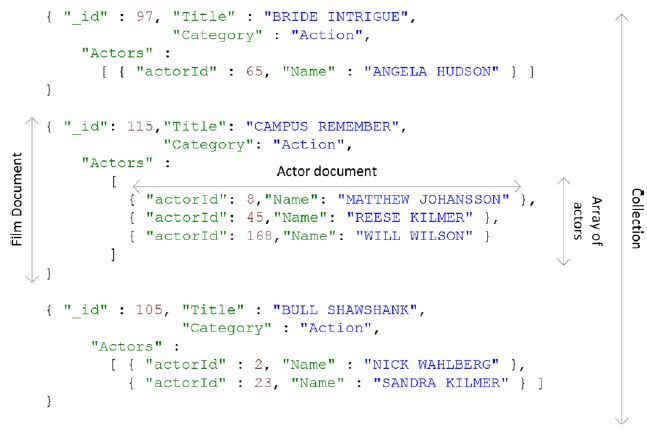
\includegraphics[scale=0.3]{images/01docstores_1.jpg}
	\caption{Beispiel eines JSON-Dokuments}\label{fig:doc1}
\end{figure}
Wie in der Abbildung \ref{fig:doc1} zu sehen, befindet sich ein Array von Schauspieler Dokumenten in dem Film Dokument. Dieser Design-Entwurf, der Document-Embedding genannt wird, hat den Vorteil, dass hierdurch auf aufwendige Join-Operationen verzichtet werden kann. Nachteil hierbei ist jedoch, dass die Schauspieler in vielen Dokumenten auftauchen und somit redundant sind. Sollte zudem eines der Schauspieler Attribute verändert werden müssen kann dies zu Inkonsistenzen führen. Ein weiteres Problem kann auftreten, wenn beispielsweise eine unbegrenzte Anzahl an Schauspielern möglich sein soll, da Dokumente in der Regel begrenzt sind. Um dieses Problem zu lösen besteht jedoch die Möglichkeit Indizes zu verwenden \cite{harrison01}.
\begin{figure}[H]
	\centering
	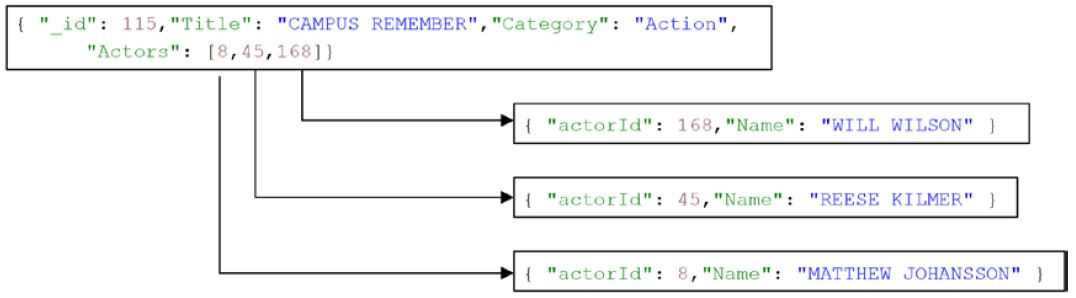
\includegraphics[scale=0.2]{images/01docstores_3.jpg} 
	\caption{Beispiel eines JSON-Dokuments}\label{fig:doc3}
\end{figure}
In Abbildung \ref{fig:doc3} ist zu sehen, wie ein solches System aussehen könnte. 
\\

Grundsätzlich gilt bei modernen Document-Stores, dass Dokumente üblicherweise in JSON bzw. BSON vorliegen \cite{harrison01}.

\subsubsection{JSON}
Die Java-Script-Object-Notation ist ein vom Menschen und Maschinen lesbarer Standard zur Beschreibung von Daten. JSON ist wie XML ein Standard zum Datenaustausch im Web.
In \ref{fig:doc1} ist ein Beispiel für ein JSON-Dokument zu sehen. Vorteil von JSON ist, dass JSON-Dokumente einfach zu zerlegen und umzuwandeln sind. Dies verringert den Aufwand, der in der Anwendungsschicht betrieben werden muss.
\subsubsection{BSON}
Unter BSON sind binär kodierte JSON-Dokumente zu verstehen. BSON erweitert das Modell von JSON um weitere Datentypen und ermöglicht effizientes kodieren und dekodieren innerhalb verschiedener Sprachen.
\subsection{Anwendungsfälle}
JSON basierte Document-Stores haben vor allem in Web-basierten Anwendungen ihre Vorzüge. Hier wird häufig JSON als Datenschicht verwendet, weswegen Document-Stores hier bevorzugt werden.
\\

XML-basierte Document-Stores finden vor allem in Content-Management-Systemen Anwendung, da sie hier ein Management Repository für XML-basierte Textdateien zur Verfügung stellen.
\\

Grundsätzlich lässt sich jedoch feststellen:
\begin{itemize}
\item dass Document-Stores vor allem in Umgebungen florieren, in denen über viele Wege Zugang zu den Daten gewährleistet werden soll, die wiederum vielfältiger Natur sein können. 
\item dass Document-Stores sinnvoll sind, wenn eine große Menge an kleinen, sich wiederholenden Schreib- und Lesevorgängen abgearbeitet werden muss.
\item dass Document-Stores sinnvoll sind, wenn die CRUD-Operationen ohne großartige Join-Operationen umgesetzt werden sollen.
\item dass Document-Stores sinnvoll sind, wenn eine programmiererfreundliche Datenbank umgesetzt werden soll.
\end{itemize}

\subsection{Bewertung}
Hieraus lässt sich evaluieren, dass Document-Stores vielfältige Einsatzmöglichkeiten haben. Vor allem im Bereich der Web-Technologien haben Document-Stores wie MongoDB Stärken, die sie zu guten Alternativen zu klassischen relationalen Datenbanken machen. Durch die Freiheiten bei den zu speichernden Daten und der Einfachheit der Abfragen zeigen sich hier vor allem ihre Stärken. Ferner wird deutlich, dass, gemessen an der Geschwindigkeit in der neue Technologien zur Darstellung von Daten entstehen, Document-Stores im Web die notwendige Freiheit bieten, um angemessen vorzugehen.

\chapter{Ausgewählte Persistenzsysteme und Big Data Frameworks}
\section{MongoDB}
\subsection{Einleitung}
Schemalose NoSQL Datenbanksysteme werden in der heutigen Zeit immer öfters verwendet, dank ihrer Flexibilität, Geschwindigkeit und Verlässlichkeit. MongoDB ist ein schemaloses Datenbanksystem, die auf Dokumentenspeicherung basiert. Diese Dokumente von MongoDB speichern die Daten in einem JSON ähnlichen, nämlich BSON (Binary JSON), was speziell für MongoDB erstellt wurde, Format. Hierbei spielt es keine Rolle, wie die Daten aufgebaut sind, die in das Dokument eingetragen werden. Dokumente in MongoDB werden in Collections gespeichert. Jede Collection fügt einem Dokument eine eindeutige ID zu.  Die Dateigröße für Dokumente beträgt maximal 16MB. Eine Ansammlung von Collections stellt die Datenbank dar.
Der Aufbau von einer Datenbank in MongoDB sieht wie folgt aus:
\\
\\
\begin{minipage}{\textwidth}
    \centering
    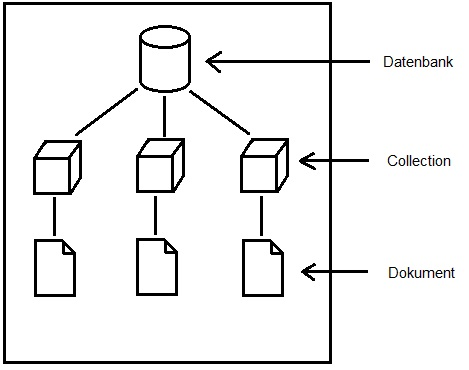
\includegraphics[scale=0.9]{images/Datenmodell_Mongo.jpg}
    \captionof{figure}{Datenbankstruktur von MongoDB}
    \label{fig:ver}
\end{minipage}
\\
Die Collection kann man wie eine Tabelle in einer relationalen Datenbank ansehen und die Dokumente sind die jeweiligen Reihen, also die konkrete Dateneintragungen in die Tabelle.
\subsection{Geschichte}
MongoDB wurde von Dwight Merriman, Eliot Horowitz und seinem Team erstellt. Doch dies nicht auf direktem Wege. 2007 plante das MongoDB Team ein Onlineservice für Web-Anwendungen. Dieser Service sollte die Möglichkeit bieten, eine Web-Anwendung zu entwickeln, zu hosten und zu skalieren. Aufgrund von einem nicht geeigneten Datenbanksystem entschloss sich das Team ein eigenes Datenbanksystem zu erstellen und zu nutzen. Diese hatte noch keinen Namen, da dieses System speziell für den Service des Teams erstellt wurde. Im Jahre 2008 wurde dann das Datenbanksystem fertiggestellt. 2009 entschloss sich das Team, dieses Datenbanksystem, was sie erstellt haben, als Open Source Produkt freizugeben. Dieses System wurde als MongoDB veröffentlicht. März 2010 kam die erste Version von MongoDB heraus, die man in einem größeren Umfang verwenden kann. Über die Jahre wurde MongoDB von dem Team weiterentwickelt und ist zurzeit mit der Version 3.2 veröffentlicht. 
\subsubsection{Philosophie}
Die Philosophie von MongoDB ist im Vergleich zu den meisten anderen etwas unterschiedlich. Denn das Team von MongoDB hat sich dazu entschieden, dass MongoDB nicht die Lösung für jedes Problem sein soll. MongoDB soll eine Lösung für Analytische Probleme und komplexe Datenstrukturen. Zudem liegt der Fokus auf die Nutzung von Dokumenten, nicht auf Zeilen. Das MongoDB Team wollte ein Datenbanksystem was sehr schnell, gut skalierbar und einfach anzuwenden ist.
\subsection{Anwendungsfälle}
MongoDB wird von verschiedenen Unternehmen zu verschiedensten Anwendungen und Aufgaben verwendet.
MTV verwendet MongoDB als Haupt-repository für das MTV-Network.
SourceForge verwendet MongoDB als Back-End Speicher.
Bit.ly verwendet MongoDB, um den Verlauf von Nutzern zu speichern.
New York Times verwendet MongoDB  für eine Foto-Abgabe.
\subsection{Einrichtung}
MongoDB wird für alle Betriebssysteme angeboten und ist derzeit in der Version 3.2 erhältlich. Dadurch lässt sich MongoDB auf Ubuntu 12.04+, Windows Server 2008+ und Mac OS X 10.7+ installieren und verwenden. 
Um MongoDB auf einem Linux Ubuntu Server zu installieren, muss man folgende Schritte befolgen:
\\
\\
1. Importierung von dem public key durch das package management System.
\\
2. Ein Listen-Datei für MongoDB erstellen.
\\
3. Lokale Dateien aktualisieren.
\\
4. Installation von MongoDB Paket.
\\
\\
Um MongoDB auf einem Windows Server zu installieren, muss man wie folgt vorgehen:
\\
\\
1. Bestimmen, welchen Build von MongoDB benötigt wird.
\\
2. MongoDB für Windows runterladen.
\\
3. Installation von MongoDB via Asministrator Kommandozeile.
\\
\\
Um MongoDB auf einem Mac OS System zu installieren, sind folgende Schritte notwendig:
\\
\\
1. Binäre Dateien von der benötigten MongoDB Version runterladen.
\\
2. Heruntergeladene Dateien extrahieren.
\\
3. Extrahierte Dateien in das Zielverzeichnis kopieren.
\\
4. Pfad von MongoDB sicherstellen.
\\
\\
Alle Vorgehensweisen für die Installation von MongoDB verwenden eine Kommandozeile.
%\subsubsection{Indexierung}
\subsubsection{Referenzierung}
Die Referenzierung von MongoDB unterscheidet sich von der Referenzierung von den relationalen Datenbanken. Eine Möglichkeit der Referenzierung in MongoDB wäre die Verschachtlung, also ein Dokument in einem Dokumenten schreiben. Damit kann man die Referenz auf ein anderes Objekt direkt erkennen, was auch für das System einfacher ist, an diese Daten zu gelangen. Das Problem hierbei kann aber eine zu starke Verschachtelungsstruktur sein, was auf Kosten der Übersichtlichkeit geht, zusätzlich wird für ein Dokument mehr Platz gebraucht, da in einem Dokument ein weiteres existiert. Die zweite Möglichkeit für eine Referenzierung, wäre der Verweis auf das jeweilige Dokument. Das verbessert die Übersicht und man kann erkennen, voraus die Daten herkommen. Ein Problem was MongoDB mit sich bringt, ist, dass es keine Direktreferenzierung gibt. In der Relationalen Datenbank kann man mit dem JOIN Befehl die Referenz zu einem anderen Datensatz in Bezug auf einen anderen Datensatz direkt ansprechen und anzeigen lassen. Dies kann MongoDB nicht. Um dies zu ermöglichen, muss man das in einer eigenen Applikation programmieren. 
\subsubsection{Replikation}
Eine Replikation bei MongoDB ist die Kopie von Daten auf weiteren Servern. Dies nennt man replica set. Ein replica set umfasst Server mit derselben Funktionalität und Dient zur Stabilisierung der Aufgabe des jeweiligen replica sets. Die MongoDB Website empfiehlt das Verwenden von drei Servern pro replica set, um somit die Ausfallrate gering zu halten. Die Daten in einem replica set sind auf allen Servern identisch. MongoDB verwendet das Master-Slave System für die Replikation von Daten innerhalb des replica sets. In dem replica set gibt es genau einen Primary und beliebig viele Secondary Server und ggf. einen Arbiter. Datenänderungen wie z.B. Schreiboperationen werden auf dem Primary Server in dem replica set durchgeführt. Nachdem die Operation erfolgreich beendet wurde, übernehmen die Secondary Server die Änderung von dem Primary Server. Sollte der Primary Server ausfallen, so wählen die Secondary Server einen neuen Primary Server aus. Man ist in der Lage, in dem replica set einen Arbiter hinzuzufügen. Ein Arbiter besitzt nicht die Daten, die in dem replica set verteilt werden. Der Arbiter dient lediglich dazu, nur bei einer Abstimmung eine Stimme abzugeben, damit eventuelle Probleme bei einer Abstimmung vermieden werden können. Ein Arbiter selber kann nicht zu einem Primary oder Secondary Server ernannt werden.
\\
\\
\begin{minipage}{\textwidth}
    \centering
    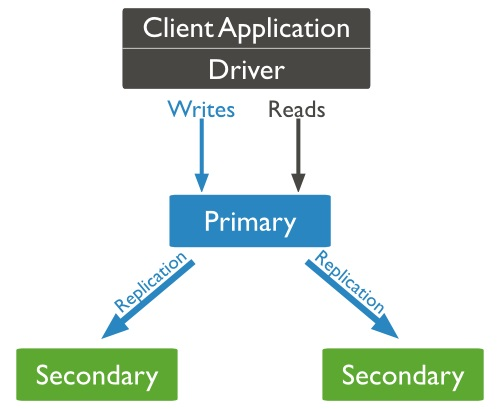
\includegraphics[scale=0.9]{images/replica-set-read-write-operations-primary.jpg}
    \captionof{figure}{Replikationsaufbau von MongoDB}
    \label{fig:ver}
\end{minipage}
\subsubsection{Cluster Sharding}
Ein sharded Cluster bei MongoDB ist eine Methode, um Daten auf unterschiedlichen Servern zu speichern und dann diese schnell aufzurufen. Ein sharded cluster besteht aus drei Komponenten: Den Config Server, den Query Server und Shards. Um ein sharded cluster einzurichten, braucht man mindestens einen Config Server, einen Query Server und 2 Shards. Dies sieht dann wie folgt aus:
\\
\\
\begin{minipage}{\textwidth}
    \centering
    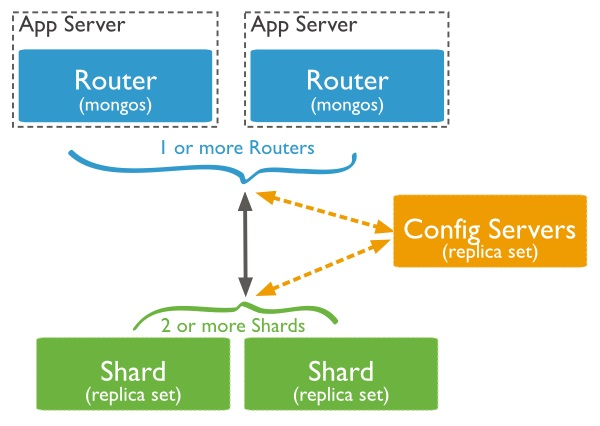
\includegraphics[scale=1.0]{images/sharded-cluster-production-architecture.jpg}
    \captionof{figure}{Aufbau vom Cluster Sharding in MongoDB}
    \label{fig:ver}
\end{minipage}
\\
\\
Config Server: Der Config Server in einem sharded Cluster beinhaltet die Metadaten für dieses. Diese Metadaten beinhalten die Informationen zu der Organisation und die Zustände der jeweiligen Komponenten in dem sharded Cluster.  Ein Config Server ist in einem replica set. Ein replica set verbessert die Konsistenz über die verschiedenen Config Server. Zusätzlich kann man danke dem replica set mehr als 3 Config Server nutzen.
Query Server (Router): Mit dem Query Server ist man in der Lage, Daten auf den verschiedenen Shards zu schreiben und zu Lesen. Dies vollbringt er mit den Metadaten, die der Query Server von dem Config Server bekommt. Der Query Server ist die einzige Schnittstelle in dem sharded Cluster, womit man auf die Daten durch Anwendungen zugreifen kann. 
\\
\\
\begin{minipage}{\textwidth}
    \centering
    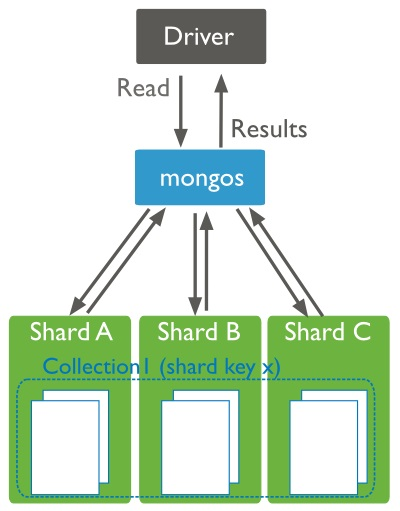
\includegraphics[scale=0.9]{images/sharded-cluster-scatter-gather-query.jpg}
    \captionof{figure}{Datenverteilung von dem Query Server}
    \label{fig:ver}
\end{minipage}
\\
\\
Shard: Bei einer Shard handelt es sich um einen Teil der Gesamtdatenbank. Die Daten, die in die Datenbank eingetragen werden, werden nach den Metadaten des Configservers analysiert und dann durch den Query Server auf das jeweilige Shard gespeichert. Zum Beispiel: Eine 3 Shard Datenbank beinhaltet Daten von Personen in einem Unternehmen. Auf Shard 1 werden alle Mitarbeiter gespeichert, die im Nachnamen mit dem Buchstaben A bis H anfangen. Shard 2 hat den Nachnamen von I bis Q und Shard 3 R bis Z. Dadurch, dass die Daten aufgeteilt und auf unterschiedlichen Shards gespeichert werden, ist man in der Lage schneller an die gewünschten Informationen zu kommen. Shards können sich in einem replica set befinden. Dieses dient für Redundanz  und hohe Verfügbarkeit der Daten.
\subsection{Verwendung}
Um mit MongoDB Daten einzufügen oder auszulesen, sind verschiedene CRUD-Operationen notwendig, wie bei einer relationellen Datenbank. Diese Operationen ähneln wie JavaScript Anweisungen und sind daher leicht anzuwenden. Die wichtigsten Befehle zur Verwendung von MongoDB sind in Tabelle 2.1 zu entnehmen.
\\
\\
\begin{table}[h]
\centering
\begin{tabular}{p{7cm}|p{7cm}|c|c|}
\hline 
Befehl & Funktion \\ 
\hline 
Use <Datenbankname> & Setzt die Datenbank zu den benutzten Namen \\ 
\hline 
db.createCollection(„Name“,{capped : true, size : <byte>, max : <anzahl> }) & Legt eine Collection mit dem angegebenen Namen \\ 
\hline 
db.<name>.insert({Name: „Thomas“, Alter: 25, …})  & Legt ein Dokument in der Collection <name> ab \\ 
\hline 
db.<name>.save({Name: „Thomas“, Alter: 22}) & Einfache Veränderung eines Dokumentes mit dem Namen “Thomas” \\ 
\hline 
db.<name>.update({Name: „Thomas“}, {Name: „Franz“ , Alter: 24}) & Veränderung eines Dokumentes mit dem Namen „Thomas“ \\ 
\hline 
db.<name>.find() & Zeigt alle Dokumente in der Collection <name> \\ 
\hline 
db.<name>.count({Name: „Franz“}) & Zählt alle Dokumente, die den Namen “Franz” beinhalten \\ 
\hline 
db.<name>.remove({Name: “Franz”}) & Löscht alle Dokumente mit dem Namen “Franz” \\ 
\hline 
db.<name>.drop() & Die Collection löschen \\ 
\hline 
\end{tabular}
\caption{Befehlsliste für MongoDB}
\end{table} 
\\
Beim Arbeiten von MongoDB sollte stets geachtet werden, dass man auf der richtigen Datenbank arbeitet und dass die Dokumente in die richtige Collections eingetragen werden. Zudem sollte man auf Groß-  und Kleinschreibung achten, da MongoDB Case-Sensitive ist. 
\subsection{Grenzen}
MongoDB besitzt in mehrere Bereiche Limitationen, die die Performance und das Nutzen von MongoDB einschränken. 
\begin{itemize}
\item 32bit Version von MongoDB kann nur eine Datenbank einrichten, die maximal 2 GB groß sein kann. Dieses Problem kann behoben werden, indem man die 64bit Version von MongoDB verwendet. Zudem wird die 32bit Version von MongoDB nicht mehr seit der 3.0 Version unterstützt.
\item BSON Dokumente können maximal 16MB groß sein, was aber in Vergleich zu anderen Datenbanksystemen sehr groß ist.
\item Indexe in MongoDB können nicht größer als 1024 Byte sein. Zudem kann eine Collection maximal 64 Indexe besitzen. Auch der Name des Indexes ist auf 128 Byte begrenzt. Diese Limitationen sollten bei einer gut aufgebauten Datenbank nicht erreicht werden.
\item Sobald eine Collection mit einer Grenze eingestellt wurde, kann diese nicht erweitert werden. Das maximum was man bei der Grenzeinstellung vornehmen kann ist 232 Dokumente. Man ist aber auch in der Lage, diese Grenze auszustellen. Sollte die Grenze erreicht werden, kann man nur mit einer neuen Collection mit einer größeren oder keiner Grenze das Problem beheben.
\item Das Sharding sollte wenn möglich so früh wie möglich eingeführt werden, da sonst die Performance von MongoDB stark beeinträchtigt wird, da die Server die Daten auf den unterschiedlichen Shards verteilen muss. Zudem sollte auch geachtet werden, das die Datenbank nicht über 256 GB groß ist, da MongoDB bei einer Größe von 256 GB das Sharding nicht mehr erlaubt.
\item Die Daten die bei MongoDB versendet werden sind nicht verschlüsselt.
Bei Lese und Schreibvorgänge bei der MongoDB muss man auf Groß- und Kleinschreibung achten, da MongoDB Case-Sensitive ist.
\item MongoDB besitzt keine JOIN-Operation. Man muss diese durch verschachtelte Dokumente oder auf einen verweis auf das jeweilige Dokument machen.
\end{itemize}
\chapter{Ausgewählte Anwendungsszenarien}
\section{Web 2.0 - Abschlussarbeiten-DB}
Im Rahmen dieses Projektes ist ein relationales Schema und eine Menge an Datens\"atzen gegeben. Ziel ist es, dieses in eine NoSQL Lösung zu übertragen und die Datens\"atze in der Datenbank zu persistieren.

\subsection{Das semantische Schema}
In der Abbildung \ref{fig:schema1} ist das Schema der Datenbank zu sehen, die in den g\"angigen NoSQL Techniken umgesetzt werden sollen. Eine Abschlussarbeit wird von einem "'Student"' oder einem "'Trainee"' geschrieben. Sowohl der "'Student"', als auch der "'Trainee"', als auch der "'Examiner"', als auch der "'Supervisor"' sind Unterklassen der Klasse "'Human"'. In Auftrag gegeben wird die Arbeit von einer "'Organisation"', die eine "'University"' oder eine "'Company"' sein kann. Die Arbeit wird eventuell von einer Menge von "'First\_Examiner"' und einer Menge von "'Second\_Examiner"' begutachtet, wenn es zu einem "'Degree"' f\"uhrt. Das mit dem "'Degree\_Topic"' verbundene "'Degree"' hat einen Titel. Das "'Topic"' kann in einer "'Topic\_Category"' liegen, in der gegebenenfalls auch der "'examiner"' oder die "'Company"' liegen. Dies bedeutet, die zentrale Klasse ist das "'Topic"', dass entweder ein "'Degree\_Topic"' oder ein "'Trainee\_Topic"' ist. Hierbei ist das "'Degree\_Topic"' wiederum entweder die "'Bachelor\_Thesis"' oder die "'Master\_Thesis"'.\\

Das Schema deutet also an, dass ein Mensch, der eine Abschlussarbeit schreibt, entweder ein Auszubildender oder ein Student ist. Diese Abschlussarbeit schreibende Person schreibt die Arbeit entweder im Rahmen einer Ausbildung oder im Rahmen eines Studiums, der mit einem Abschluss ("'Degree"') belegt ist. Fasst man dies zusammen h\"atte man eine Tabelle in der Informationen zu Abschlussarbeiten gespeichert sind. Diese enthalten neben dem "'Topic"' der Arbeit auch weitere Informationen zu den Umst\"anden. Insgesamt sind 27 Klassen gegeben, auf denen 36 Attribute verteilt sind.\\

\begin{figure}[H]
	\centering
	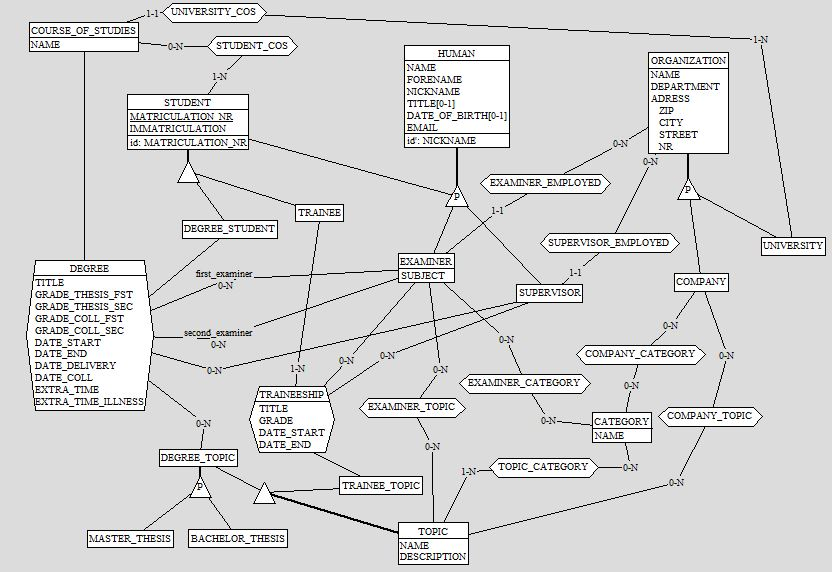
\includegraphics[scale=0.6]{images/01abschlussarbeitendbschema.jpg} 
	\caption{AbschlussarbeitenDB Schema}\label{fig:schema1}
\end{figure}

\subsection{Die Datenbestände}
Die Tats\"achlichen Daten unterscheiden sich stark von den in dem Schema \ref{fig:schema1} dargestellten Sachverhalten. Wie in Abbildung \ref{fig:schema2} zu sehen gibt es insgesamt 21 Spalten. Insgesamt umfasst die Datenbasis 1637 Datensätze. \\

\begin{figure}[H]
	\centering
	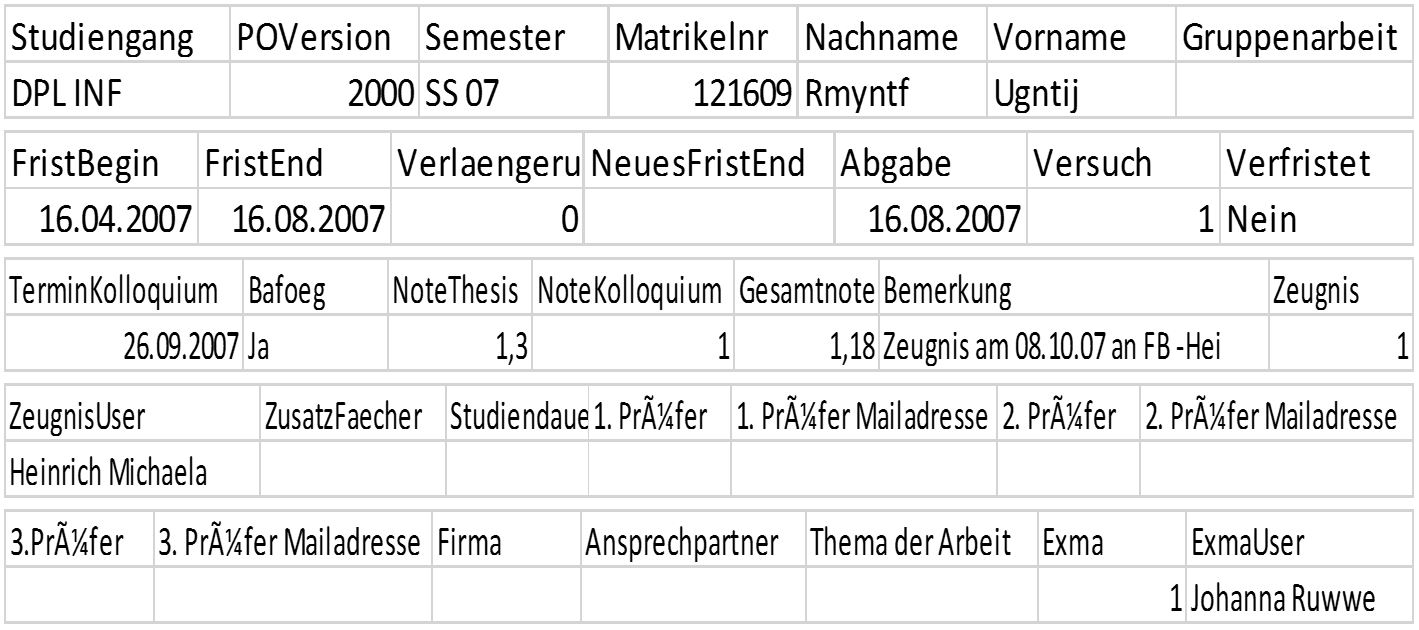
\includegraphics[scale=0.3]{images/01beispieldatensatzcsv.jpg} 
	\caption{Beispiel-Datensatz}\label{fig:schema2}
\end{figure}

Im Vergleich mit dem Schema f\"allt auf, dass es scheinbar einige Probleme gibt. Die erhobenen Daten weisen folgende Probleme auf:\\
\begin{itemize}
\item Die 21 Spalten repr\"asentieren 21 Attribute, die eine deutliche Differenz zu den 36 Attributen des Schemas darstellen. Dies bedeutet, in den Datenbest\"anden sind weniger Informationen gegeben, als eigentlich im Schema festgelegt.
\item In den Daten kommen Attribute vor, die im Schema nicht erw\"ahnt wurden. Dies umfasst Attribute wie z.B. "'Gruppenarbeit"' oder "'Bafoeg"'.
\item Einige Attribute verfügen über andere Bezeichnungen, als in dem Schema genannt werden. So hat ein Student laut Schema eine "'Matriculation\_NR"'. In den Daten ist dieses Attribut jedoch unter der Bezeichnung "'Matrikelnr"' aufgef\"uhrt.
\item In den Spalten der Daten sind einige Attribute mit Sonderzeichen belegt, was bei der \"Ubertragung der Daten in eine NoSQL Datenbank zu Problemen führen kann.
\item Einige Spalten enthalten keine Werte, was bei der \"Ubertragung der Daten in die Datenbank gegebenenfalls ber\"ucksichtigt werden muss. Besonders kritisch ist dies in den F\"allen zu sehen, bei denen das "'Thema der Arbeit"' keinen Wert hat.
\item Ein Problem der Daten ist, dass ein Professor teilweise unter verschiedenen Bezeichnungen in der Tabelle aufgeführt ist. \\
\end{itemize}

Bei der \"Ubertragung der Daten in eine Datenbank, müssen L\"osungen für die verschiedenen Probleme gefunden werden. Hier muss vor allem entschieden werden, welches Objekt bei der Migration in die NoSQL Datenbank wichtiger ist. Wird dem Schema gr\"o\ss{}ere Beachtung geschenkt, m\"ussen gr\"o\ss{}ere Anpassungen an den Daten vorgenommen werden. Sollten die Daten gr\"o\ss{}ere Priorit\"at haben, muss die Rolle des Schemas und dessen G\"ultigkeit \"uberdacht werden.\\

\subsection{MongoDB}

\chapter{Fazit}
\section{MongoDB}
Als NoSQL Datenbankl\"osung ist MongoDB vor allem f\"ur Entwickler eine Datenbank, die eine schnelle Einrichtung erm\"oglicht.\\

\subsection{Zusammenfassung}
Da die Befehle f\"ur die Interaktion mit der Datenbank JavaScript \"ahnlich waren, wurde die Arbeit mit der MongoDB vereinfacht. Die bereitgestellten Funktionalit\"aten und die ausf\"uhrliche Dokumentation der MongoDB sowie die automatische Verwaltung der Datenbank hat einen schnellen Einstieg erm\"oglicht. Durch den Java Treiber von MongoDB war es problemlos m\"oglich eine Java-basierte Web-Anwendung an die Datenbank anzubinden. Ferner hat sich gezeigt, dass die Datenbank eine \"au\ss{}erst gute Performance hat.\\ 

\subsection{Pros}
Vorteile der MongoDB sind:\\
\begin{itemize}
\item Einfache und schnelle Installation von MongoDB
\item Sehr gute Dokumentation \"uber Funktionen und Features
\item Skalierbarkeit durch Sharding
\item Geschwindigkeit
\item Flexibilit\"at
\item JSON \"ahnliche Datenformat
\end{itemize}

\subsection{Cons}
Nachteile der MongoDB sind:\\
\begin{itemize}
\item CSV-Import-Funktion ist fehlerbehaftet
\item MongoDB unterst\"utzt kein JOIN verfahren, Referenzierungen m\"ussen manuell durchgef\"uhrt werden
\item Concurrency Issues
\item Beschr\"ankungen beim Daten-Import
\end{itemize}

\subsection{Ausblick}
Die entwickelte Web-Anwendung lie\ss{}e sich weiterentwickeln und verfeinern zu einem Portal, \"uber das Studenten Informationen zu potenziellen Themengebieten, Pr\"ufern und Unternehmen finden k\"onnen. Professoren k\"onnten hier\"uber auf einfache Weise pr\"ufen, welche Themen belegt sind und an welchen Stellen Potenzial gegeben ist. Ferner k\"onnten Unternehmen das Portal nutzen, um Studenten f\"ur Abschlussarbeitsthemen zu finden. Daf\"ur m\"usste die Anwendung allerdings um weitere Funktionen, wie beispielsweise eine Login-Komponente erweitert werden um die Sicherheit zu gew\"ahrleisten.  
%Eidesstattliche Erklärung
\chapter*{Eidesstattliche Erklärung}\markboth{Eidesstattliche Erklärung}{}
  \addcontentsline{toc}{chapter}{Eidesstattliche Erklärung}
Ich versichere an Eides Statt durch meine eigenhändige Unterschrift, dass ich die entsprechend im Vorwort gekennzeichneten Abschnitte der vorliegenden Gruppenarbeit selbstständig und ohne fremde Hilfe angefertigt habe. Alle Stellen, die wörtlich oder dem Sinn nach auf Publikationen oder
Vorträgen anderer Autoren beruhen, sind als solche kenntlich gemacht.
Ich versichere außerdem, dass ich keine andere als die angegebene
Literatur verwendet habe. Diese Versicherung bezieht sich auch auf alle in
der Arbeit enthaltenen Zeichnungen, Skizzen, bildlichen Darstellungen und
dergleichen.
\\
\\
Die Arbeit wurde bisher keiner anderen Prüfungsbehörde vorgelegt und
auch noch nicht veröffentlicht.
\vspace{3cm}

\centering
\begin{tabular}{p{10mm}>{\centering\arraybackslash}p{50mm}p{10mm}
>{\centering\arraybackslash}p{50mm}p{10mm}}
&\textit{\large \TOWN,}&&& \\
&\textit{\large den \today}&&\hrulefill& \\
&\small Ort, Datum&&\small \AUTHOR&
\end{tabular}
%Zusammenfassung
\begin{abstract}
\section*{Zusammenfassung}\markboth{Zusammenfassung}{}
  \addcontentsline{toc}{chapter}{Zusammenfassung}Moderne Datenbanken sehen sich mit diversen Problemen konfrontiert. Es sollen extrem große Datenmengen verarbeitet werden und die Antwortzeiten sollen niedrig gehalten werden. Ferner soll es für sehr viele Nutzer gleichzeitig möglich sein Abfragen zu stellen. Aus diesen Gründen ist es in modernen Datenbanken notwendig ist, Datenstrukturen möglichst flexibel und performant zu speichern. Diese Probleme sollen mit verschiedenen Ansätzen aus dem Umfeld der NoSQL Datenbanksysteme gelöst werden. Die dokumentenbasierte Speicherung versucht für Probleme, welche sich meist auf große Mengen mit heterogenen Daten beziehen, einen Lösungsansatz zu finden. In diesem Umfeld ist die Funktionsweise der MongoDB äußerst populär, da sie auf hohe Leistung, große Datenmengen, hohe Flexibilität und einfache Skalierbarkeit ausgelegt ist. Die Grundlage für die der MongoDB zugrunde liegenden dokumentenbasierte Speicherung bieten die Key-Value Stores, welche unformatierte Werte unter einem Key persistieren. Document Stores vereinen den Vorteil der Schemafreiheit der Schlüssel-Wert Zuordnungen mit der Möglichkeit zur Strukturierung von Daten. Dadurch sind Datenbanken wie MongoDB in der Lage komplexere JSON ähnliche Datentypen zu verarbeiten und basierend auf ihren Attributen zu indexieren. Die hier umrissenen theoretischen Grundlagen werden detailierter beschrieben und in dem NoSQL Kontext bewertet.\\


Um die theoretischen Grundlagen zu verdeutlichen werden mithilfe eines Anwendungsszenarios die Vorteile von MongoDB verdeutlicht. Grundlage für das Anwendungsszenario ist das logische Schema einer relationalen Datenbank, in der sowohl Abschlussarbeitsthemen, als auch alle beteiligten Personen, wie beispielsweise Studenten oder Prüfer, sowie Organisationen, gespeichert sind. \\
Ziel des Anwendungsszenarios ist es, dieses Schema mit Hilfe von MongoDB umzusetzen. Ferner soll die Eignung von MongoDB in diesem Kontext analysiert und bewertet werden. Damit MongoDB in diesem Kontext bewertet werden kann, werden unter anderem Performancetests an der Datenbank durchgeführt. Weiter soll eine Web-Anwendung implementiert werden, welche die grundsätzlichen Datenbankoperationen an der MongoDB veranschaulicht.
\end{abstract}

%Anhänge
\chapter{Anhänge}
\section{Use Cases}\label{use_cases}

\paragraph{Use Case 1} Als Student möchte ich herausfinden welche Professoren in der Vergangenheit Themen unterstützt haben, die mich interessieren. \\
\textbf{Input:} Thema das mich interessiert (als String). \\
\textbf{Output:} Liste mit Professoren die im Zusammenhang mit dem Thema 1. Prüfer waren. \\
\textbf{Query:}

\begin{lstlisting}[caption={Query zu Use Case 1},language=java,captionpos=t,numbers=none, numberstyle=\tiny,basicstyle=\scriptsize,breaklines=true]
db.getCollection('abDBsimpleCSV')
	.distinct('1_Pruefer',{"Thema_der_Arbeit":/.*Thema_der_Arbeit.*/})
\end{lstlisting}\label{lst:query1}

\textbf{Quellcode:}

\begin{lstlisting}[caption={Quellcode zu Use Case 1},language=java,captionpos=t,numbers=left, numberstyle=\tiny,basicstyle=\scriptsize,breaklines=true]
public List< DBObject > getQuery1( String input )
{
    Pattern pat = Pattern.compile( input, Pattern.CASE_INSENSITIVE );
    DBObject query;
    query = new BasicDBObject( "Thema_der_Arbeit", pat );
    List< DBObject > answer = coll.distinct( "1_Pruefer", query );
    return answer;
}
\end{lstlisting}\label{lst:query1code}

\paragraph{Use Case 2} Als Student möchte ich wissen, welche Professoren Bachelor- und Masterthesen anbieten oder angeboten haben. \\
\textbf{Output:} Liste von allen Professoren. \\
\textbf{Query:}

\begin{lstlisting}[caption={Query zu Use Case 2},language=java,captionpos=t,numbers=none, numberstyle=\tiny,basicstyle=\scriptsize,breaklines=true]
db.getCollection('abDBsimpleCSV')
	.distinct('1_Pruefer',{$or:[{"1_Pruefer":{$ne:""}},
		{"2_Pruefer":{$ne:""}},{"3_Pruefer":{$ne:""}}]})
\end{lstlisting}\label{lst:query2}

\textbf{Quellcode:}

\begin{lstlisting}[caption={Quellcode zu Use Case 2},language=java,captionpos=t,numbers=left, numberstyle=\tiny,basicstyle=\scriptsize,breaklines=true]
public List< DBObject > getQuery2()
{
    DBObject nequery = new BasicDBObject( "$ne", "" );
    
    List< DBObject > obj = new ArrayList<>();
    obj.add( new BasicDBObject( "1_Pruefer", nequery ) );
    obj.add( new BasicDBObject( "2_Pruefer", nequery ) );
    obj.add( new BasicDBObject( "3_Pruefer", nequery ) );
    
    DBObject orquery = new BasicDBObject( "$or", obj );
    
    List< DBObject > answer = coll.distinct( "1_Pruefer", orquery );
    return answer;
}
\end{lstlisting}\label{lst:query2code}

\paragraph{Use Case 3} Als Student möchte wissen welche Themen in der Vergangenheit von einem bestimmten Professor angeboten wurden. \\
\textbf{Input:} Professorname. \\
\textbf{Output:} Liste mit Themen bei welchem der Professor Prüfer war. \\
\textbf{Query:}

\begin{lstlisting}[caption={Query zu Use Case 3},language=java,captionpos=t,numbers=none, numberstyle=\tiny,basicstyle=\scriptsize,breaklines=true]
db.getCollection('abDBsimpleCSV')
	.distinct('Thema_der_Arbeit',{$or:[{"1_Pruefer":"Professorname"},
		{"2_Pruefer":"Professorname"},
		{"3_Pruefer":"Professorname"}]})
\end{lstlisting}\label{lst:query3}

\textbf{Quellcode:}

\begin{lstlisting}[caption={Quellcode zu Use Case 3},language=java,captionpos=t,numbers=left, numberstyle=\tiny,basicstyle=\scriptsize,breaklines=true]
public List< DBObject > getQuery3( String input )
{
    Pattern pat = Pattern.compile( input, Pattern.CASE_INSENSITIVE );
    DBObject query;
    query = new BasicDBObject( "1_Pruefer", pat );
    List< DBObject > answer = coll.distinct( "Thema_der_Arbeit", query );
    return answer;
}
\end{lstlisting}\label{lst:query3code}

\paragraph{Use Case 4} Als Professor möchte ich mir die Anzahl der der erfolgreichen Abschlüsse für ein bestimmtes Semester ausgeben lassen. \\
\textbf{Input:} Semester. \\
\textbf{Output:} Anzahl der Abschlüsse. \\
\textbf{Query:}

\begin{lstlisting}[caption={Query zu Use Case 4},language=java,captionpos=t,numbers=none, numberstyle=\tiny,basicstyle=\scriptsize,breaklines=true]
db.abDBsimpleCSV.find({$and:[{Semester: "(Semstername)", Zeugnis: 1}]}).count()
\end{lstlisting}\label{lst:query4}

\textbf{Quellcode:}

\begin{lstlisting}[caption={Quellcode zu Use Case 4},language=java,captionpos=t,numbers=left, numberstyle=\tiny,basicstyle=\scriptsize,breaklines=true]
public int getQuery4( String input )
{
    List< DBObject > obj = new ArrayList<>();
    obj.add( new BasicDBObject( "Semester", input ) );
    obj.add( new BasicDBObject( "Zeugnis", 1 ) );
    DBObject andQuery = new BasicDBObject( "$and", obj );
    int i = coll.find( andQuery ).count();
    return i;
}
\end{lstlisting}\label{lst:query4code}

\paragraph{Use Case 5} Als Student möchte ich wissen, welche Unternehmen Bachelor- und Masterthesen betreut haben. \\
\textbf{Output:} Liste aller Unternehmen. \\
\textbf{Query:}

\begin{lstlisting}[caption={Query zu Use Case 5},language=java,captionpos=t,numbers=none, numberstyle=\tiny,basicstyle=\scriptsize,breaklines=true]
db.abDBsimpleCSV.distinct('Firma',{Firma: {$ne:""}})
\end{lstlisting}\label{lst:query5}

\textbf{Quellcode:}

\begin{lstlisting}[caption={Quellcode zu Use Case 5},language=java,captionpos=t,numbers=left, numberstyle=\tiny,basicstyle=\scriptsize,breaklines=true]
public List< DBObject > getQuery5()
{
    BasicDBObject nequery = new BasicDBObject( "$ne", "" );
    BasicDBObject query = new BasicDBObject( "Firma", nequery );
    List< DBObject > answer = coll.distinct( "Firma", query );
    return answer;
}
\end{lstlisting}\label{lst:query5code}

\paragraph{Use Case 6} Als Professor oder als Student möchte ich mir anzeigen lassen, welcher Professor bisher die meisten Abschlussarbeiten unterstützt hat. \\
\textbf{Output:} Liste mit Professoren und der Anzahl an unterstützten Abschlussarbeiten. \\
\textbf{Query:}

\begin{lstlisting}[caption={Query zu Use Case 6},language=java,captionpos=t,numbers=none, numberstyle=\tiny,basicstyle=\scriptsize,breaklines=true]
db.abDBsimpleCSV
	.aggregate([{$match:{"1_Pruefer": 
		{$not: {$size: 0}}}},
		{$unwind: '$1_Pruefer'}, 
		{$group: {_id: '$1_Pruefer', Anzahl: {$sum: 1}}}, 
		{$match: {Anzahl: {$gte: 2}}},
		{$sort: {Anzahl: -1}} ,
		{$limit:200}])
\end{lstlisting}\label{lst:query6}

\textbf{Quellcode:}

\begin{lstlisting}[caption={Quellcode zu Use Case 6},language=java,captionpos=t,numbers=left, numberstyle=\tiny,basicstyle=\scriptsize,breaklines=true]
public AggregationOutput getQuery6()
{
    List< DBObject > obj = new ArrayList<>();
    //Erstes Element der Queryliste
    Object sizeQuery = new BasicDBObject( "$size", 0 );
    DBObject neQuery = new BasicDBObject( "$not", sizeQuery );
    DBObject matchQuery = new BasicDBObject( "1_Pruefer", neQuery );
    obj.add( new BasicDBObject( "$match", matchQuery ) );
    //Zweites Element der Queryliste
    obj.add( new BasicDBObject( "$unwind", "$1_Pruefer" ) );
    //Drittes Element der Queryliste
    DBObject sumQuery = new BasicDBObject( "$sum", 1 );
    DBObject auswahlQuery = new BasicDBObject( "_id", "$1_Pruefer" ).append( "Anzahl", sumQuery );
    obj.add( new BasicDBObject( "$group", auswahlQuery ) );
    //Viertes Element der Queryliste
    DBObject anzahlQuery, greaterQuery;
    greaterQuery = new BasicDBObject( "$gte", 2 );
    anzahlQuery = new BasicDBObject( "Anzahl", greaterQuery );
    obj.add( new BasicDBObject( "$match", anzahlQuery ) );
    //Fuenftes Element der Queryliste
    DBObject sortQuery = new BasicDBObject( "Anzahl", -1 );
    obj.add( new BasicDBObject( "$sort", sortQuery ) );
    //Sechstes Element der Queryliste
    obj.add( new BasicDBObject( "$limit", 200 ) );
    AggregationOutput answer = coll.aggregate( obj );
    return answer;
}
\end{lstlisting}\label{lst:query6code}

\paragraph{Use Case 7} Als Professor möchte ich wissen, welche Themen bereits vorgeschlagen oder bearbeitet worden sind. \\
\textbf{Input:} Thema. \\
\textbf{Output:} Liste aller Themen die dem Input entsprechen. \\
\textbf{Query:}

\begin{lstlisting}[caption={Query zu Use Case 7},language=java,captionpos=t,numbers=none, numberstyle=\tiny,basicstyle=\scriptsize,breaklines=true]
db.abDBsimpleCSV.distinct('Thema_der_Arbeit',{"Thema_der_Arbeit":/.*(Thema).*/})
\end{lstlisting}\label{lst:query7}

\textbf{Quellcode:}

\begin{lstlisting}[caption={Quellcode zu Use Case 7},language=java,captionpos=t,numbers=left, numberstyle=\tiny,basicstyle=\scriptsize,breaklines=true]
public List< DBObject > getQuery7( String input )
{
    Pattern pat = Pattern.compile( input, Pattern.CASE_INSENSITIVE );
    DBObject query;
    query = new BasicDBObject( "Thema_der_Arbeit", pat );
    List< DBObject > answer = coll.distinct( "Thema_der_Arbeit", query );
    return answer;
}
\end{lstlisting}\label{lst:query7code}

\paragraph{Use Case 8} Welche Professoren haben wieviele Arbeiten zu einem Thema betreut. \\
\textbf{Input:} Stichwort zum Thema (Such-String). \\
\textbf{Output:} Anzahl Themen mit Such-String gruppiert nach Name des Profs, sortiert nach Anzahl Themen. \\
\textbf{Query:}

\begin{lstlisting}[caption={Query zu Use Case 8},language=java,captionpos=t,numbers=none, numberstyle=\tiny,basicstyle=\scriptsize,breaklines=true]
db.abDBsimpleCSV
	.aggregate([
		{$match:{"Thema_der_Arbeit":/.*datenbank*/}},
		{$match:{"1_Pruefer": {$not: {$size: 0}}}},
		{$unwind: '$1_Pruefer'},
		{$group: {_id: '$1_Pruefer', Anzahl: {$sum: 1}}},
		{$sort: {Anzahl: -1}} ,{$limit:200}])
\end{lstlisting}\label{lst:query8}

\textbf{Quellcode:}

\begin{lstlisting}[caption={Quellcode zu Use Case 8},language=java,captionpos=t,numbers=left, numberstyle=\tiny,basicstyle=\scriptsize,breaklines=true]
public AggregationOutput getQuery8( String input )
{
    List< DBObject > obj = new ArrayList<>();
    Pattern pat = Pattern.compile( input, Pattern.CASE_INSENSITIVE );
    DBObject query;
    query = new BasicDBObject( "Thema_der_Arbeit", pat );
    BasicDBObject mQuery = new BasicDBObject( "$match", query );
    obj.add( mQuery );
    DBObject sizeQuery = new BasicDBObject( "$size", 0 );
    DBObject neQuery = new BasicDBObject( "$not", sizeQuery );
    DBObject matchQuery = new BasicDBObject( "1_Pruefer", neQuery );
    obj.add( new BasicDBObject( "$match", matchQuery ) );
    obj.add( new BasicDBObject( "$unwind", "$1_Pruefer" ) );
    DBObject sumQuery = new BasicDBObject( "$sum", 1 );
    DBObject auswahlQuery = new BasicDBObject( "_id", "$1_Pruefer" ).append( "Anzahl", sumQuery );
    obj.add( new BasicDBObject( "$group", auswahlQuery ) );
    DBObject sortQuery = new BasicDBObject( "Anzahl", -1 );
    obj.add( new BasicDBObject( "$sort", sortQuery ) );
    AggregationOutput answer = coll.aggregate( obj );
    return answer;
}
\end{lstlisting}\label{lst:query8code}
%----------------------------------OUR SHIT--------------------------


\newpage

% loads the fancy pagestyle for register part
% set the pagestyle to fancy
\pagestyle{fancy}

\fancyhf{}% clear all fields
  % define the header
  \fancyhead[L]{\leftmark}% left header
  \fancyhead[R]{\HEADER}% right header
  \renewcommand{\headrulewidth}{0.4pt}% top line

  % define the footer
  \fancyfoot[L]{\AUTHOR}% left footer
  \fancyfoot[R]{\pagemark}% right footer
  \renewcommand{\footrulewidth}{0.6pt}% bottom line

  % redefine the chaptermark to have '1. Chaptername' and not 'CHAPTER 1.
  % CHAPTERNAME'
  \renewcommand{\chaptermark}[1]{\markboth{\thechapter.\ #1}{}}

% override the plain style
\fancypagestyle{plain}{%
\fancyhf{}% clear all fields
  % define the header
  \renewcommand{\headrulewidth}{0.0pt}% top line

  % define the footer
  \fancyfoot[L]{\AUTHOR}% left footer
  \fancyfoot[R]{\pagemark}% right footer
  \renewcommand{\footrulewidth}{0.6pt}% bottom line
}


% #####
% # load the appendix from the files
% #####
% \appendix
\chapter{Anhang}
Appendix
\section{Erster Teil}
\section{Zweiter Teil}
\chapter{Anhang}
Appendix


% #####
% # list of table, list of figures, and list of listings in ToC
% #####
%\newpage
%\addcontentsline{toc}{chapter}{Abbildungsverzeichnis}
%\listoffigures
%\newpage
%\addcontentsline{toc}{chapter}{Tabellenverzeichnis}
%\listoftables
%\newpage
%\addcontentsline{toc}{chapter}{Listings}
%\lstlistoflistings

% #####
% # List of Abbreviations
% #####
%\phantomsection 
%\addcontentsline{toc}{chapter}{Abkürzungsverzeichnis}
%\renewcommand\refname{Abkürzungsverzeichnis} 
%\chapter*{Abkürzungsverzeichnis}
%\begin{acronym}[RDBMS] % längste Abkürzung steht in eckigen Klammern
    \setlength{\itemsep}{-\parsep} % geringerer Zeilenabstand
    \acro{API}{Application Programming Interface}
    \acro{BASE}{Basically Available, Soft State, Eventual Consistency}
    \acro{BG}{Barahmand Ghandeharizadeh}
    \acro{CAP}{Consistency Availibiltiy Partition Tolerance}
    \acro{CLI}{Command-Line Interface}
    \acro{CPU}{Central Processing Unit}
    \acro{CRUD}{Create, Read, Update, Delete}
    \acro{DBA}{Datenbankadministrator}
    \acro{DBS}{Datenbanksystem}
    \acrodefplural{DBS}[DBS]{Datenbanksysteme}
    \acrodefplural{HDD}[HDDs]{Hard Disk Drive}
    \acrodefplural{SSD}[SSDs]{Solid State Drive}
    \acro{DNS}{Domain Name System}
    \acro{DTD}{Document Type Definition}
    \acro{GUI}{Graphical User Interface}
    \acro{HDD}{Hard Disk Drive}
    \acro{IP}{Internet Protocol}
    \acro{JDBC}{Java Database Connectivity}
    \acro{JSON}{JavaScript Object Notation}
    \acro{NoSQL}{Not only SQL}
    \acro{OLTP}{Online Transaction Processing}
    \acro{RDBMS}{Relational Database Management System}
    \acro{RFC}{Request For Comments}
    \acro{SLA}{Service Level Agreement}
    \acro{SPEC}{Standard Performance Evaluation Corporation}
    \acro{SQL}{Structured Query Language}
    \acro{SSD}{Solid State Drive}
    \acro{TPC}{Transaction Processing Performance Council}
    \acro{UML}{Unified Markup Language}
    \acro{XML}{Extensible Markup Language}
    \acro{YCSB}{Yahoo! Cloud Serving Benchmark}
\end{acronym}

%\newpage

% #####
% # load the bibliography
% #####
\bibliography{b.01}

% #####
% # load the sworn declaration
% #####
%\chapter*{Eidesstattliche Erklärung}\markboth{Eidesstattliche Erklärung}{}
  \addcontentsline{toc}{chapter}{Eidesstattliche Erklärung}
Ich versichere an Eides Statt durch meine eigenhändige Unterschrift, dass
ich die vorliegende Arbeit selbstständig und ohne fremde Hilfe angefertigt
habe. Alle Stellen, die wörtlich oder dem Sinn nach auf Publikationen oder
Vorträgen anderer Autoren beruhen, sind als solche kenntlich gemacht.
Ich versichere außerdem, dass ich keine andere als die angegebene
Literatur verwendet habe. Diese Versicherung bezieht sich auch auf alle in
der Arbeit enthaltenen Zeichnungen, Skizzen, bildlichen Darstellungen und
dergleichen.
\\
\\
Die Arbeit wurde bisher keiner anderen Prüfungsbehörde vorgelegt und
auch noch nicht veröffentlicht.
\vspace{3cm}

\centering
\begin{tabular}{p{10mm}>{\centering\arraybackslash}p{50mm}p{10mm}
>{\centering\arraybackslash}p{50mm}p{10mm}}
&\textit{\large \TOWN,}&&& \\
&\textit{\large den \today}&&\hrulefill& \\
&\small Ort, Datum&&\small \AUTHOR&
\end{tabular}
% end of the document
\end{document}
